\documentclass[border=3pt]{standalone}
% Shared preamble for the standalone figures of qurl_explained.tex.
% Build a figure from this folder:   tectonic fig_<name>.tex
% Colours: blue = full precision (FP), orange = 8-bit.
\usepackage[T1]{fontenc}
\usepackage{lmodern}
\usepackage{amsmath,amssymb}
\usepackage[dvipsnames]{xcolor}
\usepackage{tikz}
\usetikzlibrary{positioning,arrows.meta,calc,decorations.pathreplacing}
\usepackage{pgfplots}
\pgfplotsset{compat=1.17}
\colorlet{fp}{RoyalBlue}
\colorlet{qb}{BurntOrange}
\colorlet{good}{ForestGreen}
\colorlet{bad}{BrickRed}
\newcommand{\pold}{\pi_{\mathrm{old}}}
\newcommand{\thold}{\theta_{\mathrm{old}}}
\newcommand{\qthold}{\hat\theta_{\mathrm{old}}}
\tikzset{
  box/.style={draw, rounded corners=3pt, align=center, inner sep=4pt, font=\small},
  arr/.style={-{Stealth[length=2.2mm]}, thick},
  lab/.style={font=\footnotesize, align=center},
}
\pgfplotsset{
  small axes/.style={
    tick label style={font=\footnotesize}, label style={font=\footnotesize},
    title style={font=\small}, every axis plot/.append style={line join=round}},
}

\begin{document}
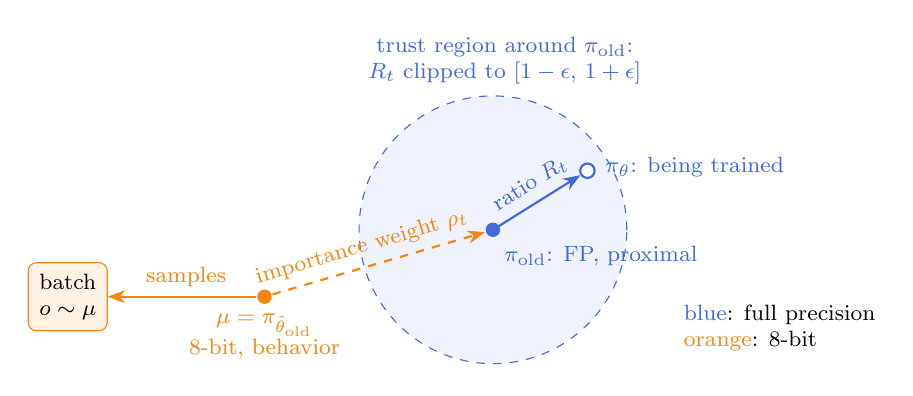
\begin{tikzpicture}[font=\small]
\coordinate (P) at (0,0);         % proximal: FP old policy
\coordinate (T) at (1.2,0.75);    % current policy
\coordinate (M) at (-2.9,-0.85);  % behavior: 8-bit policy
% trust region around the proximal policy
\fill[fp!8] (P) circle (1.7);
\draw[fp, dashed] (P) circle (1.7);
\node[fp, lab] at (0.15,2.15) {trust region around $\pold$:\\ $R_t$ clipped to $[1-\epsilon,\,1+\epsilon]$};
% proximal policy
\fill[fp] (P) circle (2.6pt);
\node[fp, lab, anchor=north west] at ($(P)+(0.02,-0.08)$) {$\pold$: FP, proximal};
% current policy
\draw[fp, thick, fill=white] (T) circle (2.6pt);
\node[fp, lab, anchor=west] at ($(T)+(0.1,0.05)$) {$\pi_\theta$: being trained};
\draw[arr, fp, shorten >=3pt] (P) -- node[lab, above, sloped] {ratio $R_t$} (T);
% behavior policy
\fill[qb] (M) circle (2.6pt);
\node[qb, lab, anchor=north] at ($(M)+(0,-0.1)$) {$\mu=\pi_{\qthold}$\\ 8-bit, behavior};
\draw[arr, qb, dashed, shorten >=3pt, shorten <=3pt] (M) -- node[lab, above, sloped, pos=0.45] {importance weight $\rho_t$} (P);
% the batch
\node[box, draw=qb, fill=qb!9, font=\footnotesize] (B) at (-5.4,-0.85) {batch\\ $o\sim\mu$};
\draw[arr, qb, shorten <=3pt] (M) -- node[lab, above] {samples} (B);
% legend
\node[lab, anchor=west, align=left] at (2.3,-1.25) {\textcolor{fp}{blue}: full precision\\ \textcolor{qb}{orange}: 8-bit};
\end{tikzpicture}
\end{document}
